\section{Redes neurais artificiais}
\label{sec:rna}
\index{MLP}
\index{RNA}
\index{Redes Neurais Artificiais}

Este trabalho é fortemente apoiado em redes neurais. Toda a fundamentação posterior possui-as como base para algo um pouco mais complexo. Portanto, um conhecimento sólido deste tópico, é um requisito indispensável. Redes neurais, de acordo com \citeonline{haykin_redes_2007}, são definidas como "[...] um processador maciçamente paralelamente distribuído constituído de unidades de processamento simples, que têm a propensão natural para armazenar conhecimento experimental e torná-lo disponível para uso." (HAYKIN, 2007, p.28). De forma simplória, uma rede neural consiste em componentes simples, que apesar de isolados não serem capazes de generalizar ou aprender complexidade exorbitante, quando organizados em conjuntos estruturados, contribuem individualmente para que a rede como um todo seja capaz de realizar tarefas mais complicadas.

Estas unidades simples de processamentos são conhecidas como \textit{neurônios artificiais} e a rede neural, é um conjunto destes neurônios interligados de uma maneira específica. Um neurônio pode ser definido como uma estrutura que possui três características básicas: um conjunto de conexões (conhecidas tecnicamente como \textit{sinapses}), uma forma de combinar sinais de entrada e uma função de ativação \cite{haykin_redes_2007}. 

As sinapses representam as conexões feitas entre neurônios e compreendem sinais de entradas sendo calibrados pelo peso da conexão. No modelo mais simples de redes neurais, esta calibração é feita em forma de multiplicação, ou seja, um sinal de entrada $x_i$ é multiplicado pelo peso sináptico $w_i$ para obtermos a sinapse $i$. Como dito anteriormente, um neurônio possui um conjunto de sinapses e os valores computados por estas precisam ser combinados de alguma forma. Uma das formas de calcular tal combinação é fazendo o simples somatório do valor das sinapses, obtendo assim uma saída para aquele neurônio. 

A função de ativação modula esta saída de acordo com a necessidade. Talvez o problema a ser resolvido requeira limitar a saída deste neurônio para um intervalo arbitrário, ou talvez converter a saída em um conjunto limitado de valores. A função de ativação é a responsável por esta tarefa. A figura \ref{fig:fig1}, descreve visualmente como um neurônio artificial é representado matemática e computacionalmente. Na imagem, os \textit{inputs} são os sinais de entrada; \textit{weights} são os pesos sinápticos; \textit{transfer function} é o combinador interno (o símbolo grego $\Sigma$ [sigma] indica um somatório); e \textit{activation function}, representada por $\upvarphi$ é a função de ativação. Para implementar esta arquitetura programaticamente, utiliza-se de operações matriciais para calcular a saída do neurônio, em relação às suas entradas ponderadas por seus respectivos pesos.

\begin{figure}[H]
    \centering
    \caption{Diagrama de um neurônio artificial.}
    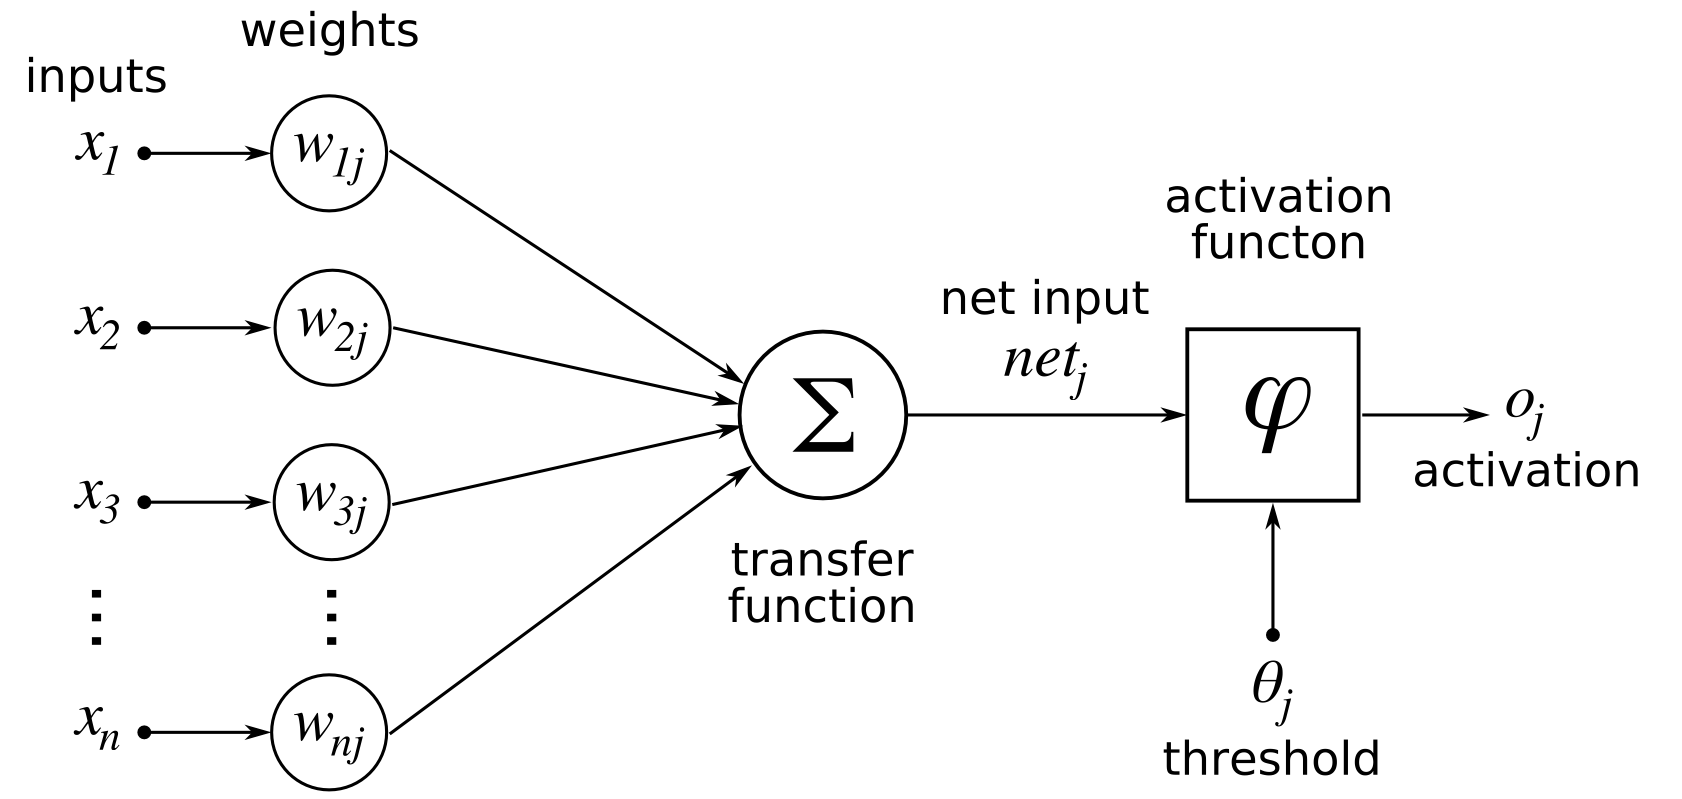
\includegraphics[width=8cm]{fig/ArtificialNeuronModel.png}
    \legend{Fonte: \cite{chrislb_english_2005}}
    \label{fig:fig1}
\end{figure}

Inspirado pela forma como nosso cérebro funciona e computa, o neurônio artificial foi primeiramente desenvolvido em 1943 por McCulloch e Pitts e ficou conhecido como \textit{modelo de McCulloch-Pitts} \cite{mcculloch_logical_1943}. Apesar de inovador, o neurônio tem suas limitações. Um único neurônio está limitado a problemas linearmente separáveis \cite{haykin_redes_2007}. Esta limitação trouxe uma estagnação na área de inteligência artificial em torno do neurônio por alguns anos. 

Posteriormente, o neurônio foi organizado em camadas, formando assim, uma rede neural onde agora, os problemas aplicáveis não precisam ser necessariamente linearmente separáveis. A imagem \ref{fig:fig2} mostra como tal estrutura de neurônios é organizada, onde \textit{hidden layer} é uma camada intermediária, ou uma camada escondida e \textit{output layer} é a camada de saída. Cada círculo representa um neurônio e as setas, a ligação entre estes.

\begin{figure}[H]
    \centering
    \caption{Diagrama de uma rede neural ou de um perceptron de múltiplas camadas.}
    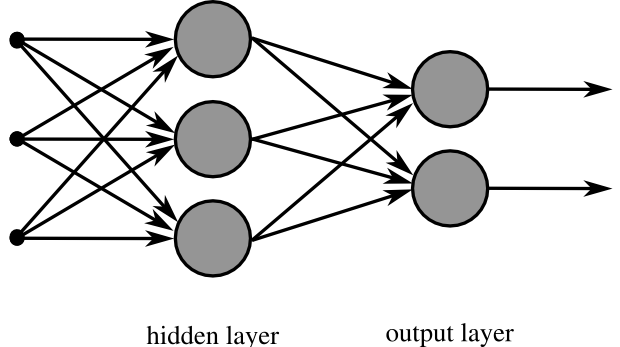
\includegraphics[width=8cm]{fig/MultiLayerNeuralNetwork_english.png}
    \legend{Fonte: \cite{wikimedia_multilayerneuralnetwork_2021}}
    \label{fig:fig2}
\end{figure}

\index{MLP} \index{Multilayer Perceptron}

O sinal de entrada desta rede, é propagado da entrada para a saída, em forma de uma série de operações matemáticas. O princípio de funcionamento do neurônio continua o mesmo: os sinais de entrada são balanceados pelo peso das ligações, combinados internamente e calibrados pela função de ativação. Agora no entanto, a saída deste neurônio é propagada para todo neurônio que recebe seu sinal de saída como entrada. Vide figura \ref{fig:fig3}. A saída do neurônio \textit{A} é propagada para todos os neurônios que possuem-a como entrada: neurônios \textit{B} e \textit{C}.

\begin{figure}[H]
    \centering
    \caption{Diagrama de uma rede neural ou de um perceptron de múltiplas camadas com fluxo de dados. }
    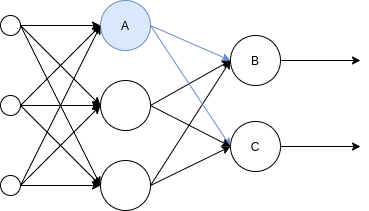
\includegraphics[width=8cm]{fig/MLP.png}
    \legend{Fonte: autor}
    \label{fig:fig3}
\end{figure}

Estas redes foram e são amplamente utilizadas para os mais diversos tipos de classificação e modelagem de dados, porém, por maior que seja sua capacidade de generalização e aprendizado, este modelo em específico é insuficiente para se capturar padrões espaciais em determinados tipos de dados. Isto é, é possível encontrar padrões entre números mas estes modelos não dependem da ordem da entrada. Caso a entrada seja uma imagem, em um perceptron de múltiplas camadas (considere uma imagem preto e branca representada como uma matriz de \textit{NxM} onde cada posição corresponde ao valor do pixel da imagem naquele local), não faz diferença se a imagem em forma de matriz for remodelada em um vetor, retirando assim uma dimensão da estrutura \cite{zhang_dive_2021}. De forma mais simples, este modelo tem dificuldades em aprender padrões que representam o relacionamento de um dado com seus adjacentes, como um pixel e a forma como este interfere com os pixels ao seu redor e por estes é afetado.
